\documentclass{standalone}
\usepackage{tikz}
\usetikzlibrary{patterns, positioning}


\begin{document}
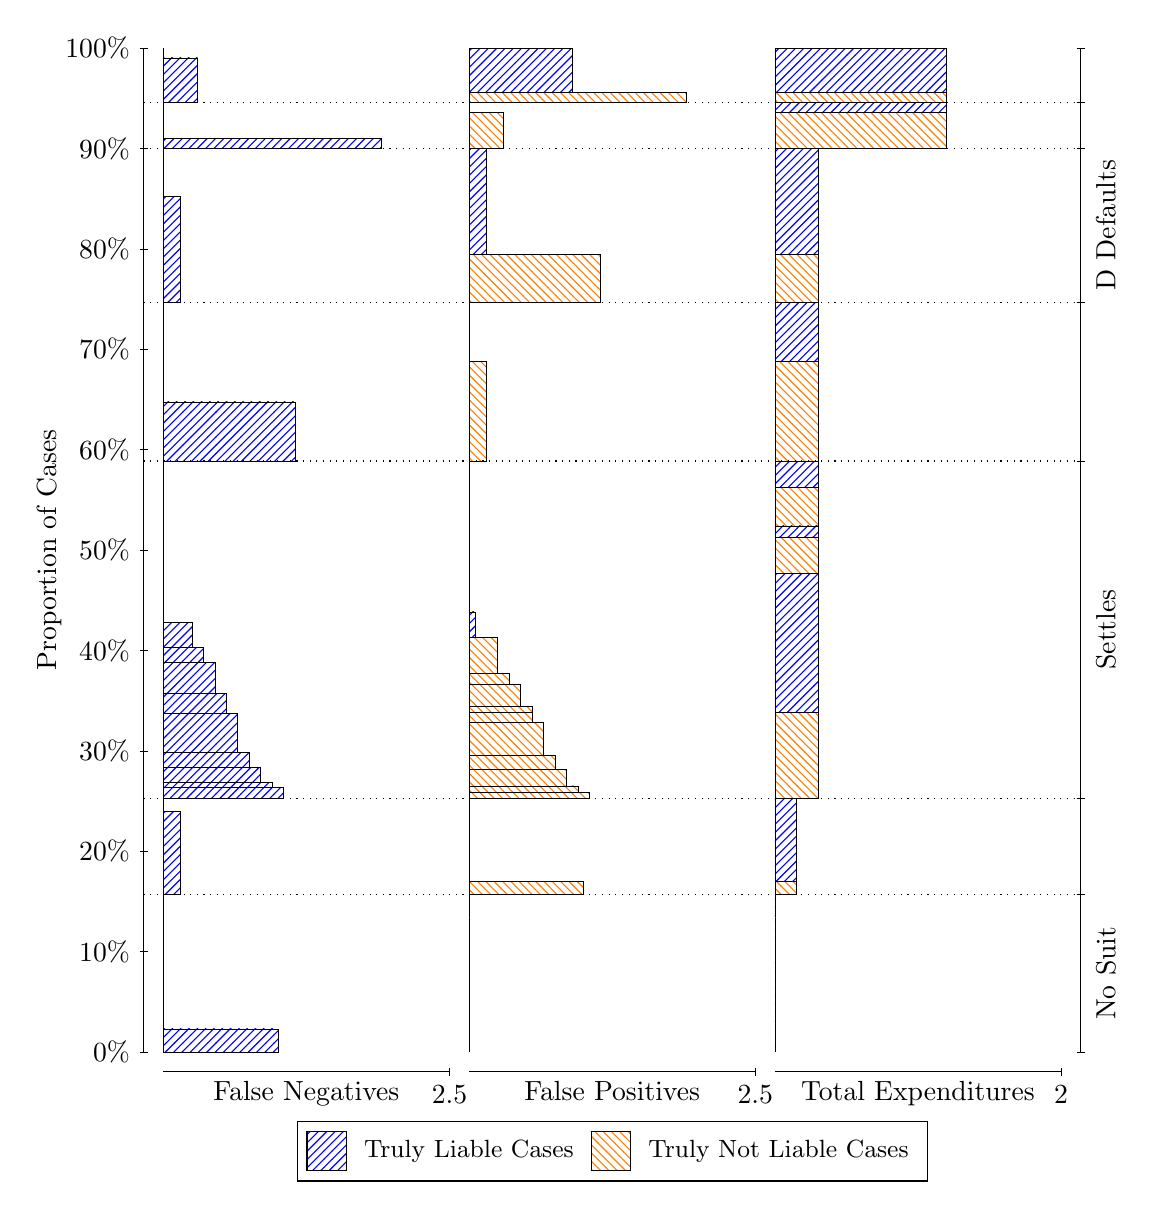
\begin{tikzpicture}
\draw[black, very thin] (1.5,1.75) -- (1.5,14.5);
\node[rotate=90, text=black, anchor=center] at (0.3, 8.125) {Proportion of Cases};
\draw[black, very thin] (1.45,1.75) -- (1.55,1.75);
\node[text=black, anchor=east] at (1.45, 1.75) {0\%};
\draw[black, very thin] (1.45,3.025) -- (1.55,3.025);
\node[text=black, anchor=east] at (1.45, 3.025) {10\%};
\draw[black, very thin] (1.45,4.3) -- (1.55,4.3);
\node[text=black, anchor=east] at (1.45, 4.3) {20\%};
\draw[black, very thin] (1.45,5.575) -- (1.55,5.575);
\node[text=black, anchor=east] at (1.45, 5.575) {30\%};
\draw[black, very thin] (1.45,6.85) -- (1.55,6.85);
\node[text=black, anchor=east] at (1.45, 6.85) {40\%};
\draw[black, very thin] (1.45,8.125) -- (1.55,8.125);
\node[text=black, anchor=east] at (1.45, 8.125) {50\%};
\draw[black, very thin] (1.45,9.4) -- (1.55,9.4);
\node[text=black, anchor=east] at (1.45, 9.4) {60\%};
\draw[black, very thin] (1.45,10.675) -- (1.55,10.675);
\node[text=black, anchor=east] at (1.45, 10.675) {70\%};
\draw[black, very thin] (1.45,11.95) -- (1.55,11.95);
\node[text=black, anchor=east] at (1.45, 11.95) {80\%};
\draw[black, very thin] (1.45,13.225) -- (1.55,13.225);
\node[text=black, anchor=east] at (1.45, 13.225) {90\%};
\draw[black, very thin] (1.45,14.5) -- (1.55,14.5);
\node[text=black, anchor=east] at (1.45, 14.5) {100\%};

\draw[black, very thin] (13.4,1.75) -- (13.4,14.5);
\draw[black, very thin] (13.35,1.75) -- (13.45,1.75);
\node[anchor=west] at (13.35, 1.75) {};
\draw[black, very thin] (13.35,3.7493) -- (13.45,3.7493);
\node[anchor=west] at (13.35, 3.7493) {};
\draw[black, very thin] (13.35,4.9728) -- (13.45,4.9728);
\node[anchor=west] at (13.35, 4.9728) {};
\draw[black, very thin] (13.35,9.2552) -- (13.45,9.2552);
\node[anchor=west] at (13.35, 9.2552) {};
\draw[black, very thin] (13.35,11.271) -- (13.45,11.271);
\node[anchor=west] at (13.35, 11.271) {};
\draw[black, very thin] (13.35,13.226) -- (13.45,13.226);
\node[anchor=west] at (13.35, 13.226) {};
\draw[black, very thin] (13.35,13.81) -- (13.45,13.81);
\node[anchor=west] at (13.35, 13.81) {};
\draw[black, very thin] (13.35,14.5) -- (13.45,14.5);
\node[anchor=west] at (13.35, 14.5) {};

\draw[black, very thin, pattern color=blue, pattern=north east lines] (1.75,1.75) rectangle (3.2033,2.0421);
\draw[black, very thin, pattern color=orange, pattern=north west lines] (1.75,2.0421) rectangle (1.75,3.7493);
\draw[black, very thin, pattern color=blue, pattern=north east lines] (1.75,3.7493) rectangle (1.968,4.8088);
\draw[black, very thin, pattern color=orange, pattern=north west lines] (1.75,4.8088) rectangle (1.75,4.9728);
\draw[black, very thin, pattern color=blue, pattern=north east lines] (1.75,4.9728) rectangle (3.276,5.1116);
\draw[black, very thin, pattern color=blue, pattern=north east lines] (1.75,5.1116) rectangle (3.1307,5.1707);
\draw[black, very thin, pattern color=blue, pattern=north east lines] (1.75,5.1707) rectangle (2.9853,5.3636);
\draw[black, very thin, pattern color=blue, pattern=north east lines] (1.75,5.3636) rectangle (2.84,5.5546);
\draw[black, very thin, pattern color=blue, pattern=north east lines] (1.75,5.5546) rectangle (2.6947,6.0454);
\draw[black, very thin, pattern color=blue, pattern=north east lines] (1.75,6.0454) rectangle (2.5493,6.2995);
\draw[black, very thin, pattern color=blue, pattern=north east lines] (1.75,6.2995) rectangle (2.404,6.6944);
\draw[black, very thin, pattern color=blue, pattern=north east lines] (1.75,6.6944) rectangle (2.2587,6.8889);
\draw[black, very thin, pattern color=blue, pattern=north east lines] (1.75,6.8889) rectangle (2.1133,7.21);
\draw[black, very thin, pattern color=orange, pattern=north west lines] (1.75,7.21) rectangle (1.75,9.2552);
\draw[black, very thin, pattern color=blue, pattern=north east lines] (1.75,9.2552) rectangle (3.4213,10.007);
\draw[black, very thin, pattern color=orange, pattern=north west lines] (1.75,10.007) rectangle (1.75,11.271);
\draw[black, very thin, pattern color=blue, pattern=north east lines] (1.75,11.271) rectangle (1.968,12.616);
\draw[black, very thin, pattern color=orange, pattern=north west lines] (1.75,12.616) rectangle (1.75,13.226);
\draw[black, very thin, pattern color=blue, pattern=north east lines] (1.75,13.226) rectangle (4.5113,13.352);
\draw[black, very thin, pattern color=orange, pattern=north west lines] (1.75,13.352) rectangle (1.75,13.81);
\draw[black, very thin, pattern color=blue, pattern=north east lines] (1.75,13.81) rectangle (2.186,14.374);
\draw[black, very thin, pattern color=orange, pattern=north west lines] (1.75,14.374) rectangle (1.75,14.5);
\draw[black, very thin, pattern color=orange, pattern=north west lines] (5.6333,1.75) rectangle (5.6333,3.4572);
\draw[black, very thin, pattern color=blue, pattern=north east lines] (5.6333,3.4572) rectangle (5.6333,3.7493);
\draw[black, very thin, pattern color=orange, pattern=north west lines] (5.6333,3.7493) rectangle (7.0867,3.9133);
\draw[black, very thin, pattern color=blue, pattern=north east lines] (5.6333,3.9133) rectangle (5.6333,4.9728);
\draw[black, very thin, pattern color=orange, pattern=north west lines] (5.6333,4.9728) rectangle (7.1593,5.0496);
\draw[black, very thin, pattern color=orange, pattern=north west lines] (5.6333,5.0496) rectangle (7.014,5.1307);
\draw[black, very thin, pattern color=orange, pattern=north west lines] (5.6333,5.1307) rectangle (6.8687,5.3364);
\draw[black, very thin, pattern color=orange, pattern=north west lines] (5.6333,5.3364) rectangle (6.7233,5.5141);
\draw[black, very thin, pattern color=orange, pattern=north west lines] (5.6333,5.5141) rectangle (6.578,5.9369);
\draw[black, very thin, pattern color=orange, pattern=north west lines] (5.6333,5.9369) rectangle (6.4327,6.0628);
\draw[black, very thin, pattern color=orange, pattern=north west lines] (5.6333,6.0628) rectangle (6.4327,6.1413);
\draw[black, very thin, pattern color=orange, pattern=north west lines] (5.6333,6.1413) rectangle (6.2873,6.4217);
\draw[black, very thin, pattern color=orange, pattern=north west lines] (5.6333,6.4217) rectangle (6.142,6.5556);
\draw[black, very thin, pattern color=orange, pattern=north west lines] (5.6333,6.5556) rectangle (5.9967,7.018);
\draw[black, very thin, pattern color=blue, pattern=north east lines] (5.6333,7.018) rectangle (5.706,7.3391);
\draw[black, very thin, pattern color=blue, pattern=north east lines] (5.6333,7.3391) rectangle (5.6333,9.2552);
\draw[black, very thin, pattern color=orange, pattern=north west lines] (5.6333,9.2552) rectangle (5.8513,10.519);
\draw[black, very thin, pattern color=blue, pattern=north east lines] (5.6333,10.519) rectangle (5.6333,11.271);
\draw[black, very thin, pattern color=orange, pattern=north west lines] (5.6333,11.271) rectangle (7.3047,11.882);
\draw[black, very thin, pattern color=blue, pattern=north east lines] (5.6333,11.882) rectangle (5.8513,13.226);
\draw[black, very thin, pattern color=orange, pattern=north west lines] (5.6333,13.226) rectangle (6.0693,13.684);
\draw[black, very thin, pattern color=blue, pattern=north east lines] (5.6333,13.684) rectangle (5.6333,13.81);
\draw[black, very thin, pattern color=orange, pattern=north west lines] (5.6333,13.81) rectangle (8.3947,13.936);
\draw[black, very thin, pattern color=blue, pattern=north east lines] (5.6333,13.936) rectangle (6.9413,14.5);
\draw[black, very thin, pattern color=orange, pattern=north west lines] (9.5167,1.75) rectangle (9.5167,3.4572);
\draw[black, very thin, pattern color=blue, pattern=north east lines] (9.5167,3.4572) rectangle (9.5167,3.7493);
\draw[black, very thin, pattern color=orange, pattern=north west lines] (9.5167,3.7493) rectangle (9.7892,3.9133);
\draw[black, very thin, pattern color=blue, pattern=north east lines] (9.5167,3.9133) rectangle (9.7892,4.9728);
\draw[black, very thin, pattern color=orange, pattern=north west lines] (9.5167,4.9728) rectangle (10.062,6.0628);
\draw[black, very thin, pattern color=blue, pattern=north east lines] (9.5167,6.0628) rectangle (10.062,7.83);
\draw[black, very thin, pattern color=orange, pattern=north west lines] (9.5167,7.83) rectangle (10.062,8.2925);
\draw[black, very thin, pattern color=blue, pattern=north east lines] (9.5167,8.2925) rectangle (10.062,8.4312);
\draw[black, very thin, pattern color=orange, pattern=north west lines] (9.5167,8.4312) rectangle (10.062,8.924);
\draw[black, very thin, pattern color=blue, pattern=north east lines] (9.5167,8.924) rectangle (10.062,9.2552);
\draw[black, very thin, pattern color=orange, pattern=north west lines] (9.5167,9.2552) rectangle (10.062,10.519);
\draw[black, very thin, pattern color=blue, pattern=north east lines] (9.5167,10.519) rectangle (10.062,11.271);
\draw[black, very thin, pattern color=orange, pattern=north west lines] (9.5167,11.271) rectangle (10.062,11.882);
\draw[black, very thin, pattern color=blue, pattern=north east lines] (9.5167,11.882) rectangle (10.062,13.226);
\draw[black, very thin, pattern color=orange, pattern=north west lines] (9.5167,13.226) rectangle (11.697,13.684);
\draw[black, very thin, pattern color=blue, pattern=north east lines] (9.5167,13.684) rectangle (11.697,13.81);
\draw[black, very thin, pattern color=orange, pattern=north west lines] (9.5167,13.81) rectangle (11.697,13.936);
\draw[black, very thin, pattern color=blue, pattern=north east lines] (9.5167,13.936) rectangle (11.697,14.5);
\draw[black, dotted] (1.5,3.7493) -- (13.4,3.7493);
\draw[black, dotted] (1.5,4.9728) -- (13.4,4.9728);
\draw[black, dotted] (1.5,9.2552) -- (13.4,9.2552);
\draw[black, dotted] (1.5,11.271) -- (13.4,11.271);
\draw[black, dotted] (1.5,13.226) -- (13.4,13.226);
\draw[black, dotted] (1.5,13.81) -- (13.4,13.81);
\draw[black, very thin] (1.75,1.5) -- (5.3833,1.5);
\node[text=black, anchor=north] at (3.5667, 1.5) {False Negatives};
\draw[black, very thin] (5.3833,1.45) -- (5.3833,1.55);
\node[text=black, anchor=north] at (5.3833, 1.45) {2.5};

\draw[black, very thin] (5.6333,1.5) -- (9.2667,1.5);
\node[text=black, anchor=north] at (7.45, 1.5) {False Positives};
\draw[black, very thin] (9.2667,1.45) -- (9.2667,1.55);
\node[text=black, anchor=north] at (9.2667, 1.45) {2.5};

\draw[black, very thin] (9.5167,1.5) -- (13.15,1.5);
\node[text=black, anchor=north] at (11.333, 1.5) {Total Expenditures};
\draw[black, very thin] (13.15,1.45) -- (13.15,1.55);
\node[text=black, anchor=north] at (13.15, 1.45) {2};

\node[text=black, centered, rotate=90] at (13.72, 2.7496) {No Suit};

\node[text=black, centered, rotate=90] at (13.72, 7.114) {Settles};

\node[text=black, centered, rotate=90] at (13.72, 12.249) {D Defaults};



\draw (7.449999999999999,1.5) node[draw=none] (baseCoordinate) {};
\begin{scope}[align=center]
        \matrix[scale=0.5, draw=black, below=0.5cm of baseCoordinate, nodes={draw}, column sep=0.1cm]{
            \node[rectangle, draw, minimum width=0.5cm, minimum height=0.5cm, pattern color=blue, pattern=north east lines] {}; &
            \node[draw=none, font=\small, text=black] (B) {Truly Liable Cases}; &
            \node[rectangle, draw, minimum width=0.5cm, minimum height=0.5cm, pattern color=orange, pattern=north west lines] {}; &
            \node[draw=none, font=\small, text=black] (B) {Truly Not Liable Cases}; \\
            };
\end{scope}

\end{tikzpicture}
\end{document}